\documentclass[a4paper,titlepage]{article}
\usepackage{frontespizio}
\usepackage[italian]{babel}
\usepackage[utf8]{inputenc}
\usepackage{usecases}
\usepackage{listings}
\usepackage{verbatim}
\usepackage{tikz}
\usepackage{pdfpages}
\usetikzlibrary{arrows,shadows} % for pgf-umlsd
\usepackage[underline=true,rounded corners=false]{pgf-umlsd}
\usepackage{enumitem}
\setitemize{noitemsep,topsep=0pt,parsep=0pt,partopsep=0pt}
\usepackage[a4paper, total={6in, 9in}]{geometry}

\lstset {
basicstyle=\small,
escapeinside=\`\`,
breaklines=true
}


\begin{document}
\begin{frontespizio}
\Universita{Verona}
\Dipartimento{Informatica}
\Corso[Laurea]{Informatica}
\Titoletto{Basi di Dati}
\Titolo{Elaborato G33\\Sistema informativo per cartelle cliniche\\di una divisione ospedaliera}

\Candidato[VR359169]{Enrico Giordano}
\Candidato[VR361121]{Cristian Pinna}

\Annoaccademico{2013-2014}
\end{frontespizio}

\tableofcontents

\newpage

\part{Progettazione Concettuale}

\vfill
    \begin{center}
	
\centerline{
    %\centering
    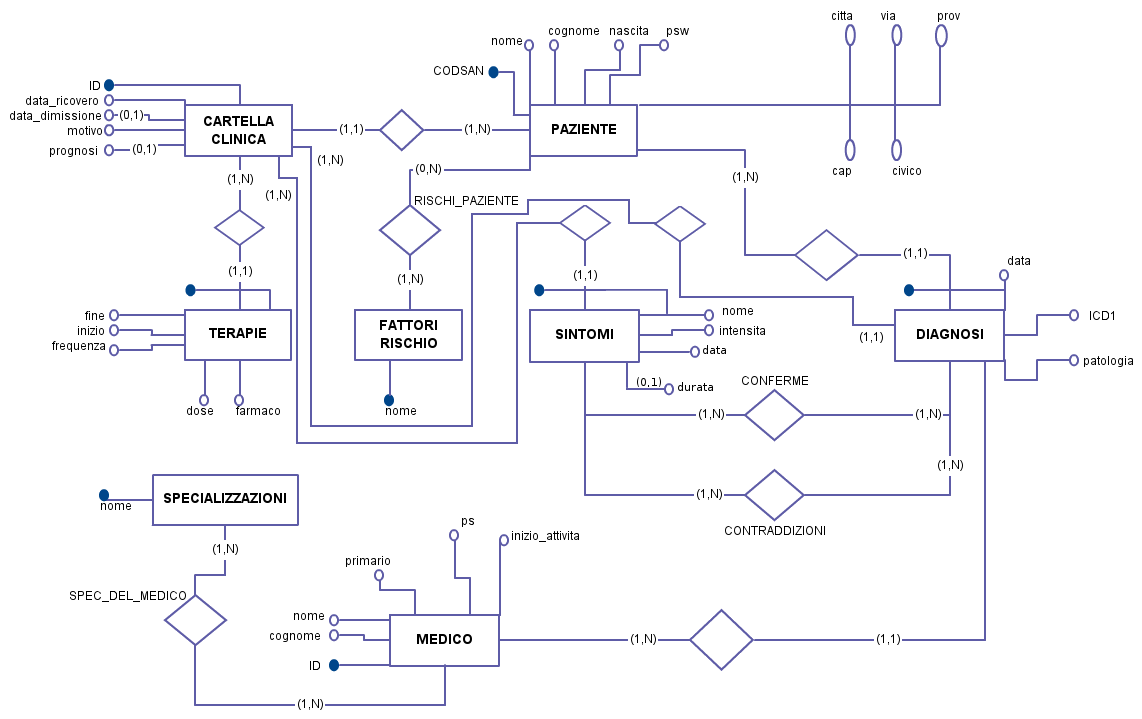
\includegraphics[scale=0.45]{ER.png}
}
    \end{center}
\vfill
\newpage
{\large Elenco delle relazioni:}\newline

\begin{enumerate}

\item Relazione TERAPIE - CARTELLA CLINICA:

\begin{itemize}[leftmargin=0.5cm, topsep=0.25cm, itemsep=0.2cm]

\item Cardinalità (1,1), una TERAPIA è associata univocamente ad una CARTELLA CLINICA
\item Cardinalità (1,N), ad una CARTELLA CLINICA può corrispondere più TERAPIE

\end{itemize}

\item Relazione CARTELLA CLINICA - PAZIENTE:

\begin{itemize}[leftmargin=0.5cm, topsep=0.25cm, itemsep=0.2cm]

\item Cardinalità (1,1), una CARTELLA CLINICA è associata univocamente ad un PAZIENTE
\item Cardinalità (1,N), ad un PAZIENTE può corrispondere più CARTELLE CLINICHE

\end{itemize}

\item Relazione CARTELLA CLINICA - SINTOMI:

\begin{itemize}[leftmargin=0.5cm, topsep=0.25cm, itemsep=0.2cm]

\item Cardinalità (1,N), ad una CARTELLA CLINICA può corrispondere uno o più SINTOMI
\item Cardinalità (1,1), un SINTOMO è associato univocamente ad una CARTELLA CLINICA

\end{itemize}

\item Relazione CARTELLA CLINICA - DIAGNOSI:

\begin{itemize}[leftmargin=0.5cm, topsep=0.25cm, itemsep=0.2cm]

\item Cardinalità (1,N), ad una CARTELLA CLINICA può corrispondere una o più DIAGNOSI
\item Cardinalità (1,1), una DIAGNOSI è associata univocamente ad una CARTELLA CLINICA

\end{itemize}

\item Relazione PAZIENTE - FATTORI RISCHIO:

\begin{itemize}[leftmargin=0.5cm, topsep=0.25cm, itemsep=0.2cm]

\item Cardinalità (0,N), ad un PAZIENTE può corrispondere nessuno o più FATTORI RISCHIO
\item Cardinalità (1,N), ad un FATTORE RISCHIO può corrispondere uno o più PAZIENTI

\end{itemize}

\item Relazione PAZIENTE - DIAGNOSI:

\begin{itemize}[leftmargin=0.5cm, topsep=0.25cm, itemsep=0.2cm]

\item Cardinalità (1,N), ad un PAZIENTE può corrispondere una o più DIAGNOSI
\item Cardinalità (1,1), una DIAGNOSI è associata univocamente ad un PAZIENTE

\end{itemize}

\item Relazione SINTOMI - DIAGNOSI:

\begin{itemize}[leftmargin=0.5cm, topsep=0.25cm, itemsep=0.2cm]

\item Cardinalità (1,N), ad un SINTOMO può corrispondere una o più DIAGNOSI
\item Cardinalità (1,N), ad una DIAGNOSI può corrispondere uno o più SINTOMI

\end{itemize}

\item Relazione DIAGNOSI - MEDICO:

\begin{itemize}[leftmargin=0.5cm, topsep=0.25cm, itemsep=0.2cm]

\item Cardinalità (1,1), una DIAGNOSI è associata univocamente ad un MEDICO
\item Cardinalità (1,N), ad un MEDICO può corrispondere una o più DIAGNOSI

\end{itemize}

\item Relazione MEDICO - SPECIALIZZAZIONI:

\begin{itemize}[leftmargin=0.5cm, topsep=0.25cm, itemsep=0.2cm]

\item Cardinalità (1,N), ad un MEDICO può corrispondere una o più SPECIALIZZAZIONI
\item Cardinalità (1,N), ad una SPECIALIZZAZIONE può corrispondere uno o più MEDICI

\end{itemize}

\end{enumerate}

\newpage

\part{Schema Logico}
    \begin{center}

    \centering
    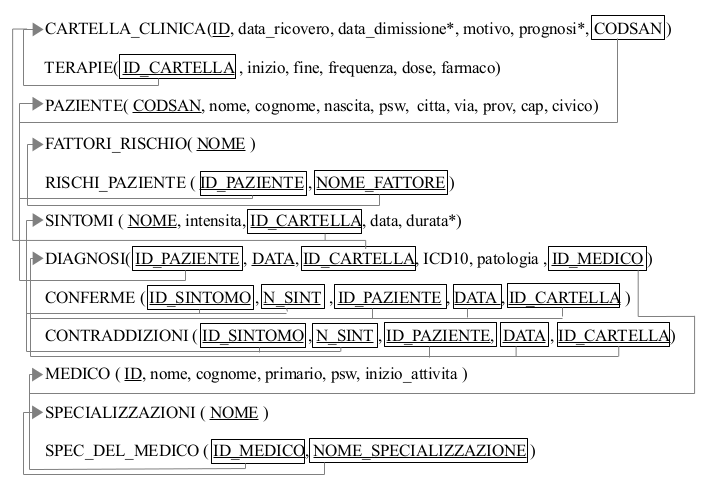
\includegraphics[scale=0.9]{schema_logico.png}

    \end{center}

Questo schema logico rappresenta una visione globale sull'elenco dei vari attributi, sulle chiavi primarie (attributi sottolineati) e sulle relazione tra di essi (i riquadri attorno al nome dell'attributo e la relativa freccia che punta alla relazione).

È stato tradotto nel file ``database.sql'' e popolato tramite il file ``popola.sql''. Quest'ultimo file esegue degli script che contengono molti insert per ogni tabella.
Per generare questi script, sono stati creati dei programmi in grado di generare file .sql con un numero considerevole di insert in base al design del database, in modo da poter testare su grandi numeri il sito (e il comportamento del database).

\newpage
\part{Page Schema}

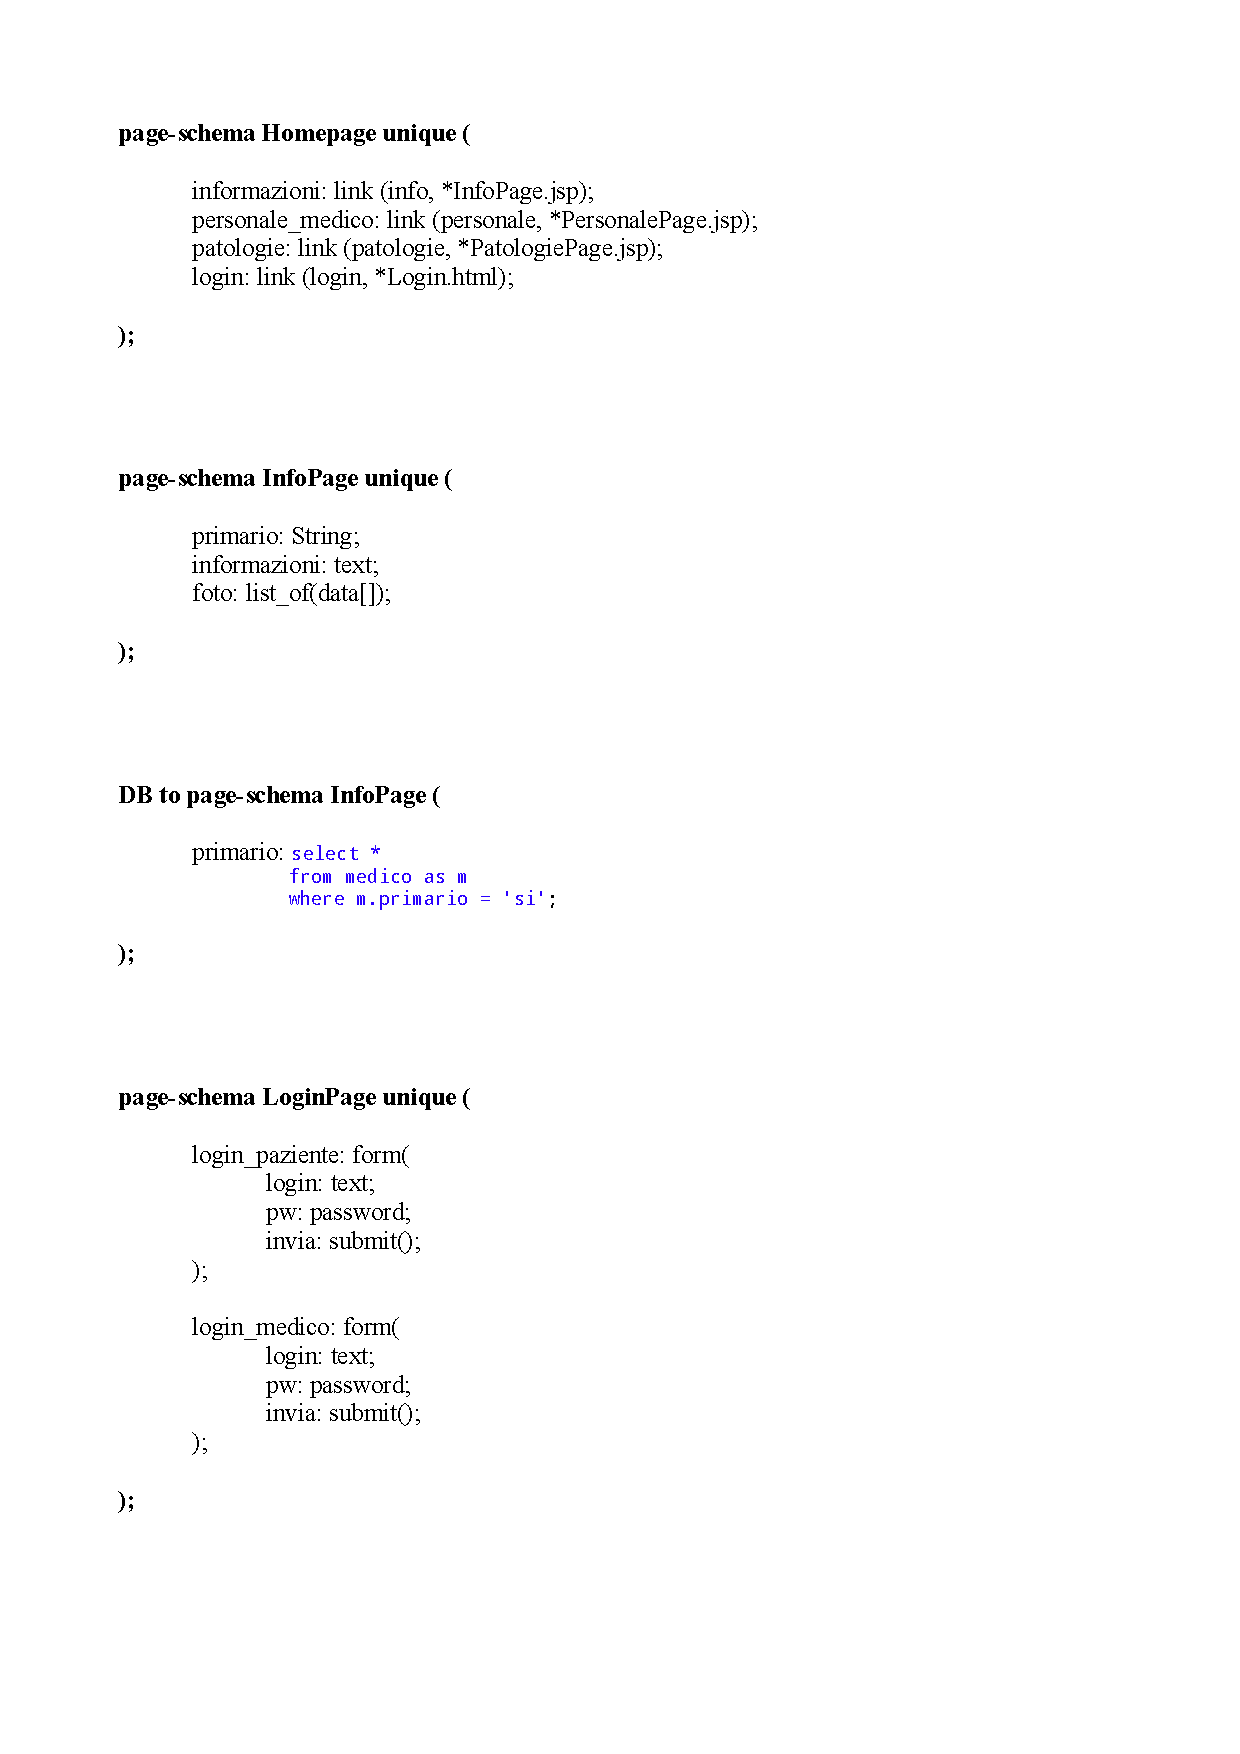
\includepdf[pages=-]{pageSchema.pdf}

\part{Strategie progettuali e considerazioni personali}

Per rendere più realistico il database, sono stati aggiunti dei vincoli sugli attributi:

\begin{itemize}[leftmargin=1.5cm, topsep=0.5cm, itemsep=0.2cm]

\item la cartella clinica deve avere una data di ricovero maggiore o uguale della data di nascita del paziente;

\item la cartella clinica deve avere una data di ricovero minore della data di dimissioni;

\item le terapie devono essere fatte in un arco di tempo compreso tra la data di ricovero e dimissione della cartella clinica corrispondente;

\item le terapie devono avere una data di inizio minore o uguale della data di fine;

\item le diagnosi devono essere fatte in un arco di tempo compreso tra la data di ricovero e dimissione della cartella clinica corrispondente.

\end{itemize}

Considerazioni personali e strategie adottate durante lo sviluppo del progetto:

\begin{itemize}[leftmargin=1.5cm, topsep=0.5cm, itemsep=0.2cm]

\item È stato resa la data dimissione (attributo della cartella clinica) come attributo opzionale in quanto si è pensato che possono esserci delle cartelle cliniche di pazienti ancora ricoverati in reparto (nonostante le specifiche non esplicitassero questo fatto);

\item Realizzazione del DB in modo tale da poter ottenere più relazioni possibili con la cartella clinica;
\item Utilizzo del metodo Hibernate durante la realizzazione del progetto in modo tale da poter semplificare le query, tenendo presente che esse restituivano tanti valori nidificati a cui ci si poteva raggiungere tramite superchiavi;
\item Durante la creazione della pagina relativa alle diagnosi (DiagnosiPage) il campo delle cartelle cliniche viene popolato tramite uno script ajax-json-jquery a seconda del paziente selezionato, in modo tale da evitare l'inserimento manuale di una cartella clinica potenzialmente errata;
\item Per la realizzazione generale della pagina web che gestisce l'intero progetto ci siamo sentiti di renderla più gradevole graficalmente inserendo uno stile di impaginazione html in formato css;
\item ECLIPSE pls!

\end{itemize}


\part{Tecnologie aggiuntive utilizzate}

\section{Hibernate}

Hibernate è un sistema o piattaforma middleware che offre un'interfaccia tra programmatore e database in modo da semplificare e gestire al meglio in maniera trasparente il database da interrogare o aggiornare. Questo sistema, tramite classi Java che rappresentano le entità del database, permette di avere un mapping tra variabili delle classi e attributi delle entità; in questo modo si può avere accesso agli attributi del database lavorando con i metodi get e set sulle variabili interessate.

Il mapping è reso possibile tramite file xml che chiarificano al sistema come mappare sia gli attributi delle entità sia le relazioni con la rispettiva cardinalità.

~

La progettazione si è incentrata sulla corretta scrittura dei file xml e delle relative classi; si è cercato inoltre di esplicitare quali fossero gli identificatori raggruppandoli in sottoclassi(qualora ce ne fossero più di uno), in modo da rendere ancora più chiara la programmazione: ogni classe avrà una dichiarazione sia di attributi sia di identificatori (quindi la creazione di una sottoclasse).

~

Oltre agli attributi e agli identificatori, si è deciso di associare la classe referenziata tramite attributo esterno alla classe interessata; in questo modo si può avere accesso a tutti i campi della classe referenziata applicando i metodi get e set alla sottoclasse, presente quindi nella classe interessata come variabile instanziata.

~

Come esempio pratico, la classe CartellaClinica ha i seguenti attributi:

\begin{lstlisting}

	private String id;
	private Paziente paziente;
	private Date dataRicovero;
	private Date dataDimissione;
	private String motivo;
	private String prognosi;
	private Set terapies = new HashSet(0);
	private Set diagnosis = new HashSet(0);
	private Set sintomis = new HashSet(0);

\end{lstlisting}

Come si può notare, la referenza all'entità Paziente (tramite attributo ``codsan'' nel modello relazionale) è resa tramite la dichiarazione della variabile paziente; quindi tramite una singola interrogazione di una specifica cartella clinica si possono sapere anche i campi del rispettivo paziente associato ad essa.

~

Come metodo di verifica della correttezza della progettazione per il sistema Hibernate, è stato utilizzato un plugin di Eclipse chiamato JBoss Tools, che contiene diverse features per Hibernate e permette di verificare la correttezza sia dei file xml sia delle classi Java a partire dalla descrizione del database.

Bisogna notare inoltre che le relazioni molti-a-molti hanno prodotto una referenza tradotta in Java con un HashSet, in modo da poter aver accesso ad ogni valore semplicemente di questo tipo di entità applicando i metodi set e get a questi HashSet. Questo si è rilevato di notevole importanza in quanto, per sapere la quantità di elementi di un certo tipo associati ad una entità, è bastato vedere la grandezza di questi HashSet utilizzando il metodo size, senza quindi fare un'ulteriore query. È stato necessario però forzare il sistema, in alcuni casi, ad avere un comportamento non ``lazy'', quindi impostando a false tale attributo nel file xml, in modo da caricare in memoria anche le istanze referenziate tramite le relazioni e quindi avere libero accesso ad esse. 

\section{Ajax JSON e JQuery}

\end{document}


